\documentclass[12pt,english]{article}
\usepackage[T1]{fontenc}
\usepackage[utf8]{luainputenc}
\usepackage{geometry}
\geometry{verbose,tmargin=1.5cm,bmargin=1.5cm,lmargin=1.5cm,rmargin=1.5cm}
\usepackage{graphicx}
\usepackage{amssymb}

\usepackage{caption}

\usepackage{xcolor}
\usepackage{subcaption}

\makeatletter



\newcommand{\lyxdot}{.}
\newcommand{\stcomment}[1]{{\color{red} st: #1}}

\makeatother

\author{ }

\usepackage{babel}
\date{}
\begin{document}

\title{MISO Problem: Two Information Sources with Coupling}

\maketitle

\section{Mathematical Formulation}

We consider an optimization problem with two information sources
\[
\mbox{min}_{\left(x_{1},x_{2},x_{3}\right)\in A}f_{2}\left(f_{1}\left(x_{1},x_{3}\right),x_{2},x_{3}\right)
\]
where $A$ is the feasible compact set and $f_{1},f_{2}$ are continuous
functions (see Figure~\ref{fig:fig1}). 



\begin{figure}[htp]
\centering
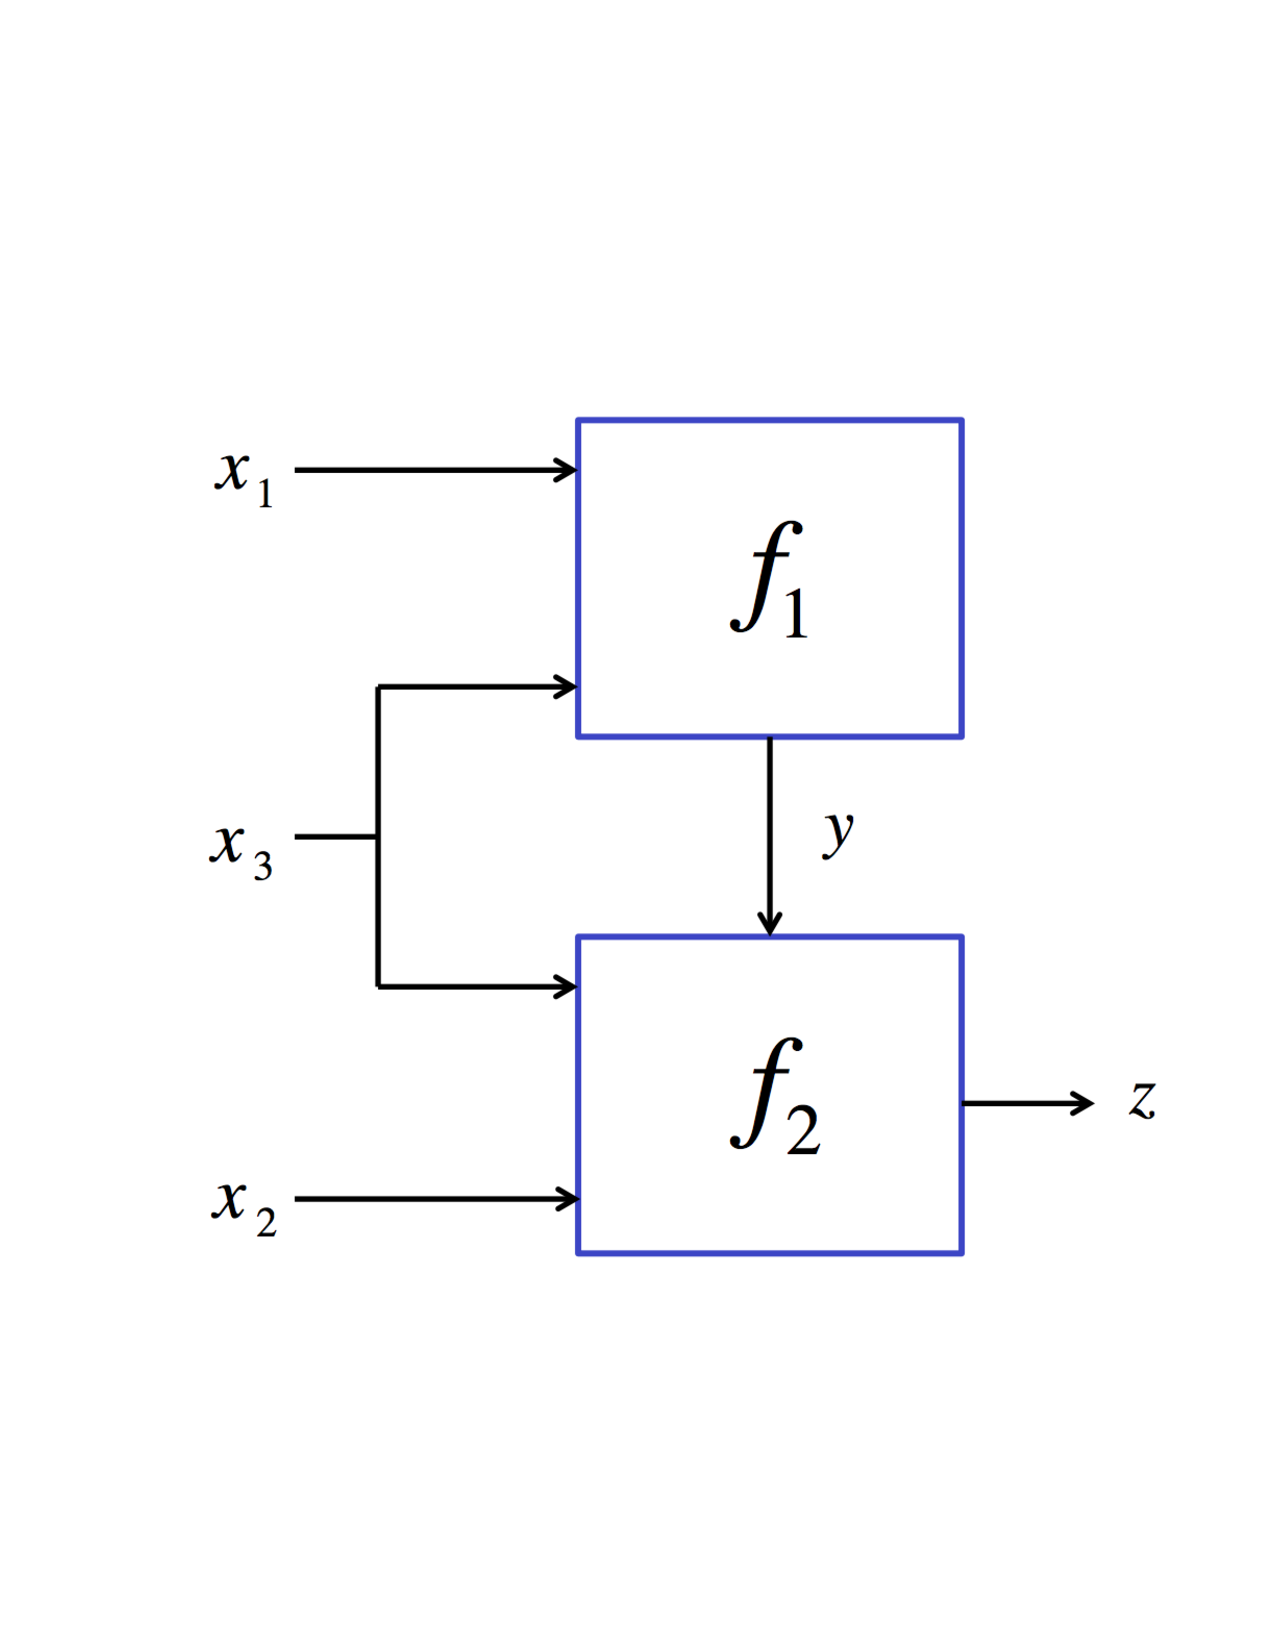
\includegraphics[width=.5\textwidth]{01.pdf}
\caption{Diagram of the problem}
\label{fig:fig1}
\end{figure}


This formulation can be used to solve different problems. For example,
$f_{1}$ could be an aerodynamic simulation of a wing and $f_{2}$
could be a structural simulation of a wing, that includes aerodynamical
forces.

\section{Value of Information Functions and Gaussian Processes}

We place two Gaussian processes on $f_{1}$ and $f_{2}$. Depending on the problem and the kernels of the Gaussian processes, we may have a Gaussian process
on $f_{2}\left(f_{1}\left(x_{1},x_{3}\right),x_{2},x_{3}\right)$ with parameters $\mu_{0}$ and $\Sigma_{0}$.

%\stcomment{Note: I think that the computations depend on the problem because the hyperparameters of the GP on the objective are computed by (the 1-dimension case):
%\begin{eqnarray*}
%p\left(f_{2}\left(f_{1}\left(x_{1},x_{3}\right),x_{2},x_{3}\right)=r\right) & = & \int_{z}p\left(f_{2}\left(f_{1}\left(x_{1},x_{3} \right),x_{2},x_{3}\right)=r\mid f_{1}\left(x_{1},x_{3}\right)=z\right)p\left(f_{1}\left(x_{1},x_{3}\right)=z\right)dz\\
% & = & \int_{z}\frac{1}{\sqrt{2\pi\Lambda_{0}\left(\left(z,x_{2},x_{3}\right),\left(z,x_{2},x_{3}\right)\right)}}e^{-\frac{\left(r-\rho_{0}\left(z,x_{2},x_{3}\right)\right)^{2}}{2\Lambda_{0}\left(\left(z,x_{2},x_{3}\right),\left(z,x_{2},x_{3}\right)\right)}}\\
% &  & \times\frac{1}{\sqrt{2\pi\beta_{0}\left(\left(x_{1},x_{3}\right),\left(x_{1},x_{3}\right)\right)}}e^{-\frac{\left(z-\alpha_{0} \left(x_{1},x_{3}\right)\right)^{2}}{2\beta_{0}\left(\left(x_{1},x_{3}\right),\left(x_{1},x_{3}\right)\right)}}dz
%\end{eqnarray*}
%}.

We define the value of information functions as

\[
V_{n}\left(x,h\right)=\mathbb{E}\left[\mbox{max}_{z}\mu_{n+1}\left(z\right)-\mbox{max}_{z}\mu_{n}\left(z\right)\mid x_{n+1}=x,h\left(x\right)\right]
\]

where $h\in\left\{f_{1},f_{2}\right\} $ and $x\in A\bigcup B$ where $B$ is the range of  $f_{1}$, which is defined by $B=\{f\left(x_{1},x_{3}\right):\exists x_{2}\mbox{ s.t }\left(x_{1},x_{2},x_{3}\right)\in A\}$.

\section{Algorithm}
\begin{enumerate}
\item (First stage of samples) Use maximum likelihood or maximum a posteriori estimation to fit the
parameters $\alpha_{0}\left(\cdot\right),\beta_{0}\left(\cdot,\cdot\right)$
of the GP prior on $f_{1}$, and $\rho_{0}\left(\cdot\right),\Lambda_{0}\left(\cdot,\cdot\right)$
of the GP prior on $f_{2}$. We denote the parameters of GP on $f_{2}\left(f_{1}\left(x_{1},x_{3}\right),x_{2},x_{3}\right)$ by
$\mu_{0},\Sigma_{0}$

\textrm{}\\
\item (Main stage of samples) For $n\leftarrow0$ to $N$ do
\begin{enumerate}
    \item Update our joint Gaussian process posterior on $f_{2}\left(f_{1}\left(x_{1},x_{3}\right),x_{2},x_{3}\right)$ using all samples by time $n$.\\
    \textrm{}\\
\item Solve $\left(x_{n+1},h_{n+1}\right)\in\mbox{arg max}_{x,h\in\left\{ f_{1},f_{2}\right\} }V_{n}\left(x,h\right)$\\
\textrm{}\\
\item Evaluate $h_{n+1}\left(x_{n+1}\right)$\\
\textrm{}\\
\end{enumerate}
\item Return $x^{*}=\mbox{arg max}_{\left(x_{1},x_{2},x_{3}\right)}\mu_{N+1}\left(x_{1},x_{2},x_{3}\right)$.


 \end{enumerate}

\end{document}
